% !TEX encoding = UTF-8 Unicode
\documentclass[a4paper]{article}

\usepackage{color}
\usepackage{url}
\usepackage[T2A]{fontenc} % enable Cyrillic fonts
\usepackage[utf8]{inputenc} % make weird characters work
\usepackage{graphicx}

% \usepackage[english,serbian]{babel}
\usepackage[english,serbianc]{babel} %ukljuciti babel sa ovim opcijama, umesto gornjim, ukoliko se koristi cirilica

\usepackage[unicode]{hyperref}
\hypersetup{colorlinks,citecolor=green,filecolor=green,linkcolor=blue,urlcolor=blue}

\newtheorem{primer}{Пример}[section] %ćirilični primer
% \newtheorem{primer}{Primer}[section]

\usepackage{listings}
\definecolor{mygreen}{rgb}{0,0.6,0}
\definecolor{mygray}{rgb}{0.5,0.5,0.5}
\definecolor{mymauve}{rgb}{0.58,0,0.82}

\usepackage{etoolbox}
\apptocmd{\sloppy}{\hbadness 10000\relax}{}{}

\usepackage{pifont}% http://ctan.org/pkg/pifont
\newcommand{\cmark}{\ding{51}}%
\newcommand{\xmark}{\ding{55}}%

\usepackage{makecell}
\usepackage{diagbox}

\lstset{ 
  backgroundcolor=\color{white},   % choose the background color; you must add \usepackage{color} or \usepackage{xcolor}; should come as last argument
  basicstyle=\scriptsize\ttfamily,        % the size of the fonts that are used for the code
  breakatwhitespace=false,         % sets if automatic breaks should only happen at whitespace
  breaklines=true,                 % sets automatic line breaking
  captionpos=b,                    % sets the caption-position to bottom
  commentstyle=\color{mygreen},    % comment style
  deletekeywords={...},            % if you want to delete keywords from the given language
  escapeinside={\%*}{*)},          % if you want to add LaTeX within your code
  extendedchars=true,              % lets you use non-ASCII characters; for 8-bits encodings only, does not work with UTF-8
  firstnumber=1000,                % start line enumeration with line 1000
  frame=single,	                   % adds a frame around the code
  keepspaces=true,                 % keeps spaces in text, useful for keeping indentation of code (possibly needs columns=flexible)
  keywordstyle=\color{blue},       % keyword style
  language=Python,                 % the language of the code
  morekeywords={*,...},            % if you want to add more keywords to the set
  numbers=left,                    % where to put the line-numbers; possible values are (none, left, right)
  numbersep=5pt,                   % how far the line-numbers are from the code
  numberstyle=\tiny\color{mygray}, % the style that is used for the line-numbers
  rulecolor=\color{black},         % if not set, the frame-color may be changed on line-breaks within not-black text (e.g. comments (green here))
  showspaces=false,                % show spaces everywhere adding particular underscores; it overrides 'showstringspaces'
  showstringspaces=false,          % underline spaces within strings only
  showtabs=false,                  % show tabs within strings adding particular underscores
  stepnumber=2,                    % the step between two line-numbers. If it's 1, each line will be numbered
  stringstyle=\color{mymauve},     % string literal style
  tabsize=2,	                   % sets default tabsize to 2 spaces
  title=\lstname                   % show the filename of files included with \lstinputlisting; also try caption instead of title
}

% Keywords command
\providecommand{\keywords}[1]
{
  \small	
  \textbf{\textit{Кључне речи ---}} #1
}

\begin{document}

\title{Упоредни преглед дебагера\\ \small{Семинарски рад у оквиру курса\\Верификација софтвера\\ Математички факултет}}

\author{Оливера Поповић, 1029/2020\\ o.popovic@outlook.com}
\maketitle

\abstract{
Како је прављење багова, односно грешака и недостатака система,
неизоставни део процеса програмирања, веома је битно постојање 
алата за њихово проналажење и уклањање. Дебагери су управо то,
сложени софтверски алати који пружају помоћ у решавању и анализи оваквих проблема.
У овом раду читалац ће имати прилику да се упозна са основим могућностима модерних дебагера, као и са 
неколико одабраних дебагера за различите системе, језике и платформе.
Изложене су специфичности сваког од њих, а приказан је и сумирани преглед њихових функционалности и могућности.
}

\keywords{дебаговање, дебагери, могућности дебагера, поређење дебагера, специфичности дебагера}

\tableofcontents

\newpage
\setlength{\parskip}{1em}

\section{Uvod}
\label{sec:uvod}

9. септембра 1947. године, тим информатичара са универзитета Харвард
пријавио је први светски \textbf{баг} (eng. ~{\em bug}) у рачунару \cite{firstBug}.
Термин баг данас се користи да означи грешку или недостатак система. 
Ипак, овај први баг био је баг у пуном значењу речи, што преведено са
енглеског језика значи буба. Наиме, тим са Харварда приметио је да 
њихов рачунар, који је био познат под називом {\em Mark II}, константно 
пријављује необичне грешке. Након што су
отворили рачунар, унутра су као узрок грешкама пронашли заглављеног 
мољца, који је пореметио електронику рачунара. Први светски баг у 
рачунару приказан је на слици \ref{fig:bug}. Ипак, ово није био
први баг пријављен у смислу техничке грешке. Томас Едисон пријавио је
багове у својим дизајнима још у 19. веку. Ово је, дакле, једино био 
први светски баг у рачунару. Чак је и Грејс Хопер, чланица поменутог
тима којој се најчешће приписују заслуге за откривање овог термина,
изјавила у једном свом интервјуу да она није створила тај термин, већ
да се он уклопио у терминологију која је већ била у употреби \cite{firstBug}.

\begin{figure}
    \begin{center}
        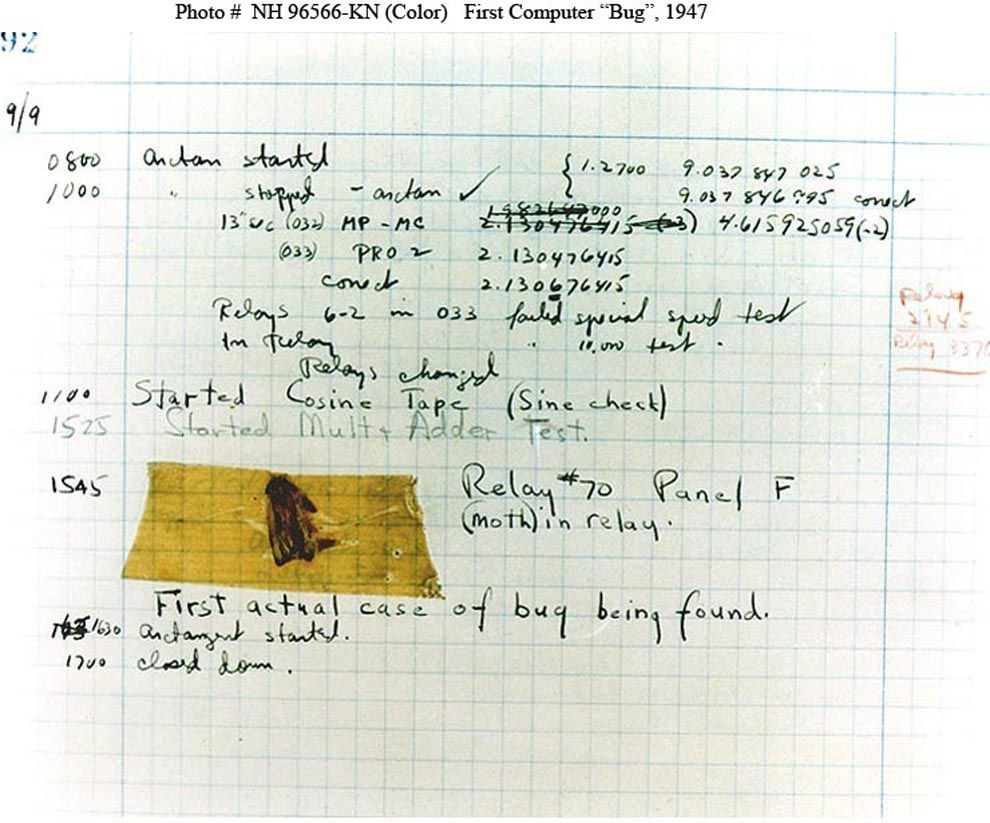
\includegraphics[scale = 0.25]{slike/prvi_bag.jpg}
    \end{center}
    \caption{Прва светскa буба (eng. ~{\em bug}) у рачунару}
    \label{fig:bug}
\end{figure}

Претходно поменути информатичари били су први који су заправо 
дебаговали рачунар. \textbf{Дебаговање} је процес проналажења и исправљања
познатих, али и потенцијалних багова у софтверу ради добијања
очекиваних резултата. Да би процес дебаговања могао бити успешан, неопходно
је добро познавање пројекта и имплементационог програмског језика,
технологија и оперативног система на ком се извршава 
програм. За отклањање неких посебно дубоко скривених грешака понекад 
је чак потребно и познавање платформе или процесора који се користи \cite{debuggingApplications}.

\break

\textit{„Ако је дебаговање процес отклањања софтверских грешака, онда
програмирање мора бити процес ниховог стварања”\\
\hspace*{0pt}\hfill-Едзгер Дејкстра}

Програми се могу дебаговати коришћењем за то посебно направљених
алата који се зову \textbf{дебагери}. Ови алати представљају комплексан
софтвер који захтева подршку компајлера, асемблера, линкера, као и оперативног
система да би исправно радили \cite{debuggersForProgrammingLanguages}.
Користе се онда када програм током извршавања не производи очекивано
понашање, а разлог за то није одмах јасан. Дебагери се
такође некада користе и да се програм интерактивно извршава,
како би се лакше разумео код који се посматра.

\section{Шта могу дебагери?}
\label{sec:whatCanDebuggersDo}

Дебагери се у процесу развоја софтвера користе од самог почетка, 
када је програм још у фази дизајна и када постоји мало написаног
кода, па све до тренутка када се софтвер испоручује корисницима \cite{debuggersForProgrammingLanguages}.
Чак и након тога, дебагери се користе од стране програмера који 
одржавају и унапређују систем, како би они разумели све 
специфичности програмског кода. Како је листа употребе веома дугачка, неопходно
је да дебагери пруже брз и ефикасан рад, али и једноставну употребу.

Главна функционалност дебагера је контрола тока извршавања програма 
који се дебагује. Најчешће коришћене опције које нуди дебагер за то
су постављање \textbf{тачака прекида} (eng.~{\em breakpoints}) 
и извршавање програма до тих тачака прекида, као
и \textbf{извршавање корак по корак} (eng.~{\em single stepping}) на нивоу наредбе, функције или
инструкције \cite{debuggersForProgrammingLanguages}.

Тачке прекида подржане су тако што се у део кода који треба 
да се изврши умеће посебан код (инструкција прекида или нека 
друга инструкција која није валидна) \cite{debuggingTechniques}. Када се приликом извршавања
дође до тог дела кода долази до прекида, који се пријављује 
дебагеру посредством процесора или оперативног система. 
Како би то било могуће, већина модерних
процесора и оперативних система поседује уграђене 
могућности које дебагери користе.
Тачке прекида могу бити и такозване условне тачке прекида (eng.~{\em conditional breakpoints}).
Оне омогућавају да се извршавање прекине уколико
је дефинисани израз евалуиран као тачан.

Функционалности које се подразумевају на модерним
дебагерима су праћење вредности променљивих (бафера, параметара, поља) и 
стања на стеку приликом извршавања, као и праћење стека позива функција.
Још неке занимљиве могућности модерних дебагера су:
\begin{itemize}
 \item Праћење вредности које се налазе у регистрима
 \item Евалуација разних израза
 \item Мењање вредности променљивих у току извршавања - што је 
       корисно јер се након измене извршавање наставља, што штеди 
       време јер је иначе потребан циклус измена-компилација
 \item Могућност наставка извршавања са друге локације,
       како би се, на пример, избегла грешка
 \item Праћење трансакција
 \item Праћење животног века (креирања и уништавања) 
       динамички алоцираних инстанци
 \item Праћење изузетака
 \item Постављање тачке посматрања (eng. ~{\em watchpoint}) - праћење вредности на одређеној 
       меморијској локацији уз могућност заустављања при свакој промени
 \item Дебаговање у вишенитним процесима
 \item Дебаговање оптимизованог кода
\end{itemize}

Дебагери подржавају и неколико различитих техника дебаговања, у које спадају \cite{debuggingTechniques}:
\begin{itemize}
 \item Интерактивно дебаговање је техника која обухвата комуникацију са дебагером,
       односно постављање тачака прекида, извршавање, паузирање и сличне опције
       за контролу тока програма
 \item Обрнуто дебаговање је техника која омогућава програмеру да сачува све
       активности програма (сваки меморијски приступ, израчунавање...) и да онда
       унатраг испита стање програма
 \item Удаљено дебаговање је поступак дебаговања програма који се извршава на
       систему који је удаљен од самог дебагера, те он за повезивање користи мрежу
 \item Посмртно дебаговање (eng.~{\em post-mortem debugging}) је поступак дебаговања
       након што се десио прекид програма
\end{itemize}


\section{Преглед дебагера}
\label{sec:debuggerOverview}

Модерни алати за развој софтвера попут развојних окружења често нуде
могућност да се комуникација са дебагером врши кроз графички кориснички
интерфејс развојног окружења или имају дебагер директно интегрисан у
окружење. Постоје и варијанте у којима разни текстуални едитори
(Visual Studio Code, Vim, Emacs...) који подржавају прикључке\footnote{Софтвер који се интегрише у постојећи
софтвер са наменом да прошири или обогати његове функционалности.} (енг. plugin) 
омогућавају повезивање са разним дебагерима докле год постоји адекватни
прикључак који испуњава интерфејс наметнут од стране едитора.

Треба истаћи да се услед овога термин дебагер у рачунарству често користи да означи
и комплетан софтверски пакет интегрисан у развојно окружење
који укључује графички кориснички интерфејс, систем за комуникацију са дебагером 
и слично, али користи се и да означи дебагер који ови претходни системи
користе да реализују свој рад. Некада и сам тај систем за дебаговање
подржава и коришћење из графичког окружења. Дакле, важно
је истаћи да постоји вишезначност у употреби овог термина. На пример развојно окружење
\texttt{QtCreator} користи дебагер \texttt{GDB} (eng. GNU Debugger)
да би кориснику пружио функционалност дебаговања.
У овој ситуацији правилније је рећи да \texttt{QtCreator} користи
\texttt{GDB} дебагер уместо да \texttt{QtCreator} има дебагер, али ни једно ни друго
нису погрешни.

У даљем тексту ће бити изложени и анализирани неки од познатијих дебагера.
У њиховом опису ће такође бити и посвећена пажња претходно споменутој
вишезначности поводом употребе термина уколико за тим буде било потребе.

\begin{figure}
    \begin{center}
        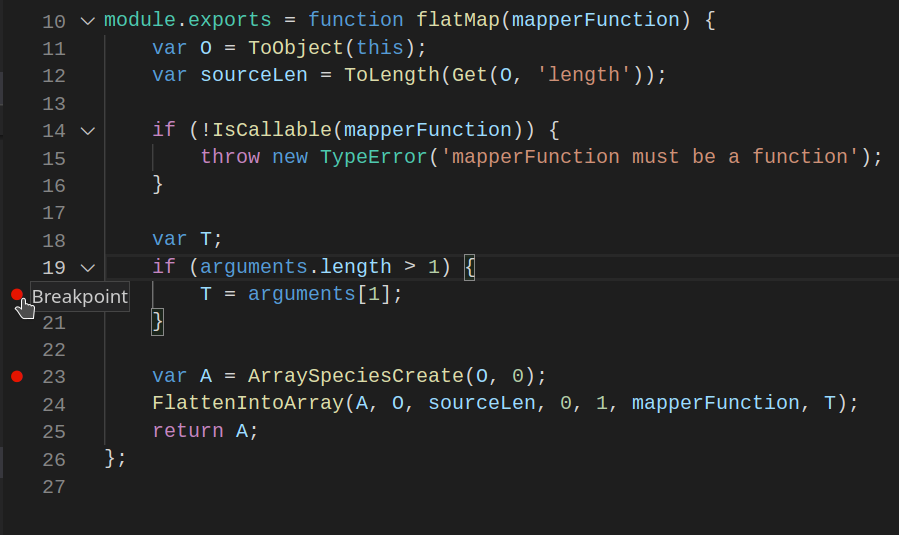
\includegraphics[scale=0.5]{slike/tacke_prekida_vscode.png}
    \end{center}
    \caption{Пример постављања тачке прекида у развојном окружењу
        {\em Visual Studio Code}}
    \label{fig:breakpoints}
\end{figure}

Интегрисани дебагери визуелно су јаснији и једноставнији за употребу из угла корисника.
За постављање тачака прекида користи се развојно окружења
(пример постављања дат је на слици \ref{fig:breakpoints}) и у тренутку 
када програм стане са извршавањем,
контрола се враћа у едитор на место које је изазвало прекид рада.
Посебно су згодни за кретање корак по корак кроз код,
јер корисник може то кретање визуелно да испрати у прозору који садржи 
изворни код програма.
Још једна погодност оваквих дебагера је то што су структуре података
компајлера доступне дебагеру, као што је на пример таблица симбола. 
Такође, уколико је потребна евалуација неких израза то ће бити 
изведено коришћењем истог компајлера који је и генерисао код, што чини 
програм конзистентним \cite{debuggersForProgrammingLanguages}.

Са друге стране, коришћење дебагера путем командне линије такође има 
своје предности. На пример, уколико је потребно нешто брзо проверити
у коду, покретање неког развојног окружења било би исувише захтевно,
па је употреба оваквих алата који се покрећу чак и неколико пута брже 
веома значајна. Још једна веома важна употреба је за дебаговање које
се врши на некој удаљеној машини путем командне линије.
У таквим ситуацијама графички кориснички интерфејс можда уопште није 
доступан, или ако јесте може бити веома спор, па је употреба кроз 
командну линију неопходна \cite{artOfDebugging}. Дебагери који омогућавају
овакав начин рада су такође и погодни за интеграцију у друге скрипте и алате
попут {\em Bash} скрипти.

Данас постоји мноштво дебагера за различите програмске језике и платформе, 
како комерцијалних тако и бесплатних, при чему неки тврда да могу 
да препознају на стотине различитих проблема.
Неколико одабраних познатих, али и мање познатих дебагера биће изложено у наставку.
Редослед излагања дебагера пратиће учесталост појављивања појединачних
дебагера у референтним изворима.

\subsection{GDB}
\label{sec:gdb}

{\em GNU} дебагер (GDB) представља један од најчешћих коришћених алата за дебаговање међу
програмерима на {\em Unix} системима \cite{artOfDebugging}. Има дугу традицију и оригинална
верзија датира још из 1986. године.
{\em GDB} пружа интерфејс за коришћење из командне линије и подржава језике
{\em C, C++, D, Fortran, Pascal, Modula-2} и {\em Ada} \cite{gdb}.
Од поменутих језика данас су најчешће у употреби C, C++ и D
па је и {\em GDB} типично најчешће асоциран као дебагер за те језике.

{\em GDB} је имплементиран у програмском језику {\em C} и поседује
{\em GPLv3} лиценцу, тако да припада групи програма отвореног кода.
На већини {\em Unix} система долази или већ инсталиран, или је доступан
као системски пакет који се једноставно може преузети и инсталирати.
Пошто је у питању софтвер отвореног кода, доступан је и на другим
платформама као што су {\em Windows}, {\em MacOS} и {\em Android}. 
Управо захваљујући томе, програм који се дебагује коришћењем овог 
алата може се извршавати на истој машини као и сам дебагер, а може
се и извршавати и на некој удаљеној машини.

\begin{figure}
    \begin{center}
        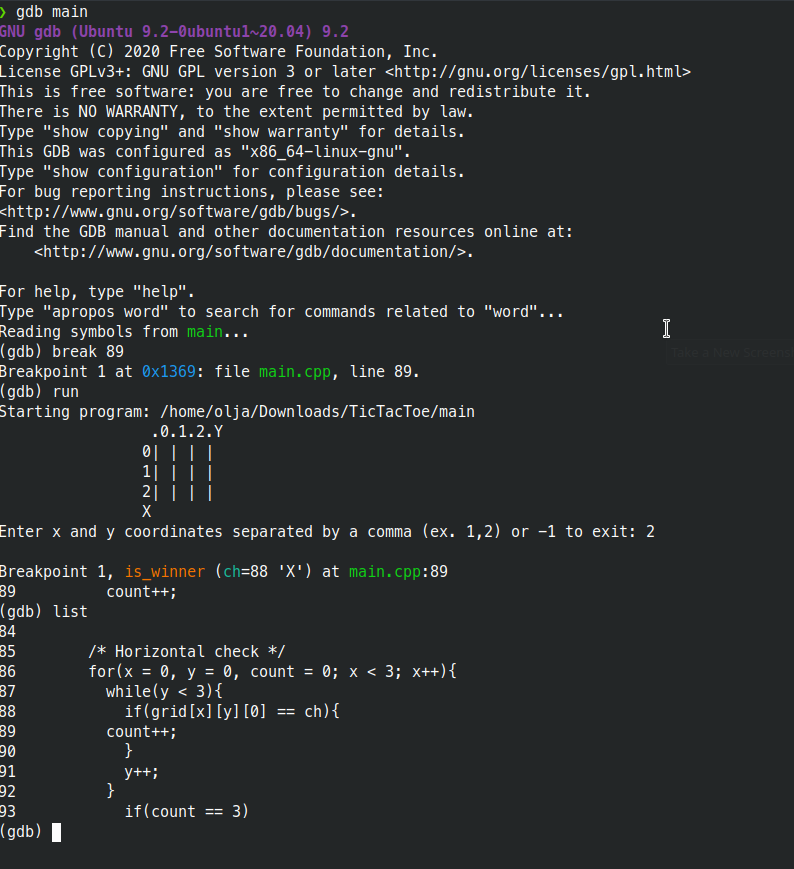
\includegraphics[scale=0.4]{slike/gdb.png}
    \end{center}
    \caption{Пример коришћења {\em GNU} дебагера}
    \label{fig:gdb}
\end{figure}

Приликом коришћења {\em GNU} дебагера постоји неколико начина за 
паузирање извршавања програма \cite{artOfDebugging}. То су
постављање тачака прекида као и условних тачака прекида, постављање тачака
посматрања, али и постављање тачака хватања. Тачке хватања (eng. ~{\em catchpoint}) 
користе се да означе да је потребно паузирати извршавање када се деси неки очекивани догађај.
Пример коришћења овог дебагера кроз командну линију дат је на 
слици \ref{fig:gdb}.

Иако овај алат не поседује сопствени графички кориснички интерфејс,
за њега је развијено неколико програма који нуде управо то.
Један од најпознатијих је \textbf{\em DDD} (eng. ~{\em Data Display Debugger}) \cite{artOfDebugging}.
Поред {\em GNU} дебагера, подржава још неколико дебагера међу којима су 
{\em DBX, WDB, Ladebug, JDB, XDB, bashdb} и {\em pydb} \cite{ddd}. 
Приказ екрана изгледа овог програма дат је на слици \ref{fig:ddd}.
Овај алат може се користити примарно на {\em UNIX} системима.
Постоји још много графичких корисничких интерфејса који су развијени 
за {\em GDB}, међу којима су \textbf{\em KDbg} (намењен системима који
користе {\em KDE} графичко окружење), затим \textbf{\em Nemiver} и \textbf{\em gdbgui}.

Као што је већ поменуто, дебагери се често користе као део већих
интегрисаних развојних окружења (eng ~{\em IDE}), па је тако {\em GDB}
такође део неколико њих, међу којима су {\em CLion, Eclipse, Qt Creator, Xcode, Dev-C++, Lazarus} \cite{gdbGui}.

\begin{figure}
    \begin{center}
        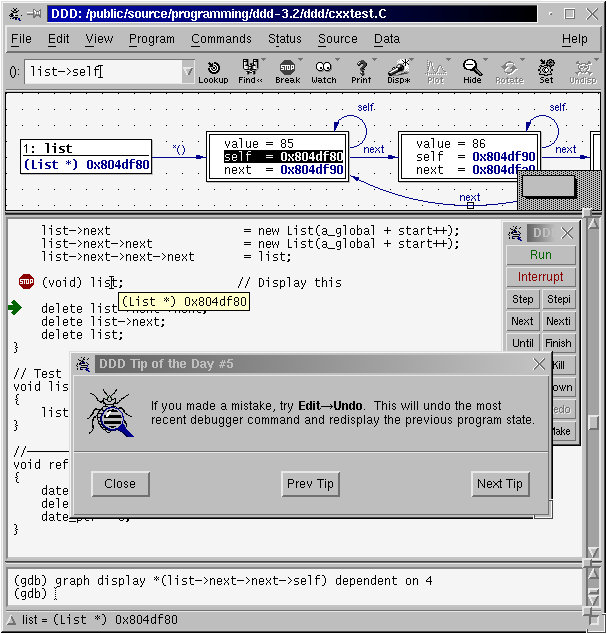
\includegraphics[scale=0.4]{slike/ddd.png}
    \end{center}
    \caption{Изглед графичког корисничког окружења {\em DDD}}
    \label{fig:ddd}
\end{figure}

\subsection{LLDB}

\textbf{\em LLVM} је пројекат отвореног кода који се развија у циљу 
пружања алата за развој софтвера као што су компилатори, алати
за анализу кода, дебагери, профајлери и линкери и слично \cite{llvm}.

\textbf{\em LLDB} је модерни дебагер који је изграђен од скупа
компоненти које у великој мери користе библиотеке овог пројекта,
као што је на пример {\em Clang} предњи део компајлера за програмске
језике из {\em C} породице језика \cite{lldb}.
{\em LLDB} има подршку за коришћење из командне линије. Чињеница да
користи {\em Clang} инфраструктуру му омогућава да подржава најновије
верзије програмских језика {\em C, C++, Objective-C} и {\em Objective-C++}.

{\em LLDB} је имплементиран у програмском језику {\em C++} и поседује
{\em Apache 2.0} лиценцу што га, као и {\em GDB}, убраја у групу 
програма отвореног кода. У тренутку писања рада, документација 
наводи постојање подршке за платформе {\em Linux, Windows, macOS, iOS, 
tvOS, watchOS} и {\em FreeBSD} \cite{lldb}. Овај алат такође нуди могућност
извршавања на удаљеним машинама, односно на машинама које се разликују
од оне на којој се извршава сам дебагер.

Неке од занимљивих особина овог алата су могућност дебаговања уназад,
постављање тачака посматрања, инспекција стања и вредности променљивих 
и још много других. Такође, {\em LLDB} покушава да користи {\em JIT} 
технике за евалуацију израза увек када је то могуће. {\em JIT} компилација
је начин извршавања кода која укључује компилацију током извршавања, а не
пре извршавања \cite[Chapter~10]{jit}.
Коришћењем алата {\em SWIG} \cite{swig}, који се користи
за повезивање програма или библиотека написаних на језицима {\em C} или
{\em C++} са скрипт језицима, програмском језику {\em Python} омогућен је
приступ и контрола јавног апликационог програмског интерфејса библиотеке 
за дебаговање \cite{lldb}.

Овај дебагер користи се као подразумевани у званичном развојном окружењу
платформе {\em macOS} које се зове {\em Xcode}. Пример употребе овог окружења
дат је на слици \ref{fig:xcode}. {\em Android Studio} такође 
користи {\em LLDB} за дебаговање \cite{android}. {\em LLDB} се може користити
и кроз многа друга интегрисана развојна окружења и едиторе, међу којима су {\em Visual
Studio Code, Eclipse} и {\em CLion}. За {\em Visual Studio Code} постоји 
прикључак под називом {\em CodeLLDB}.

\begin{figure}
    \begin{center}
        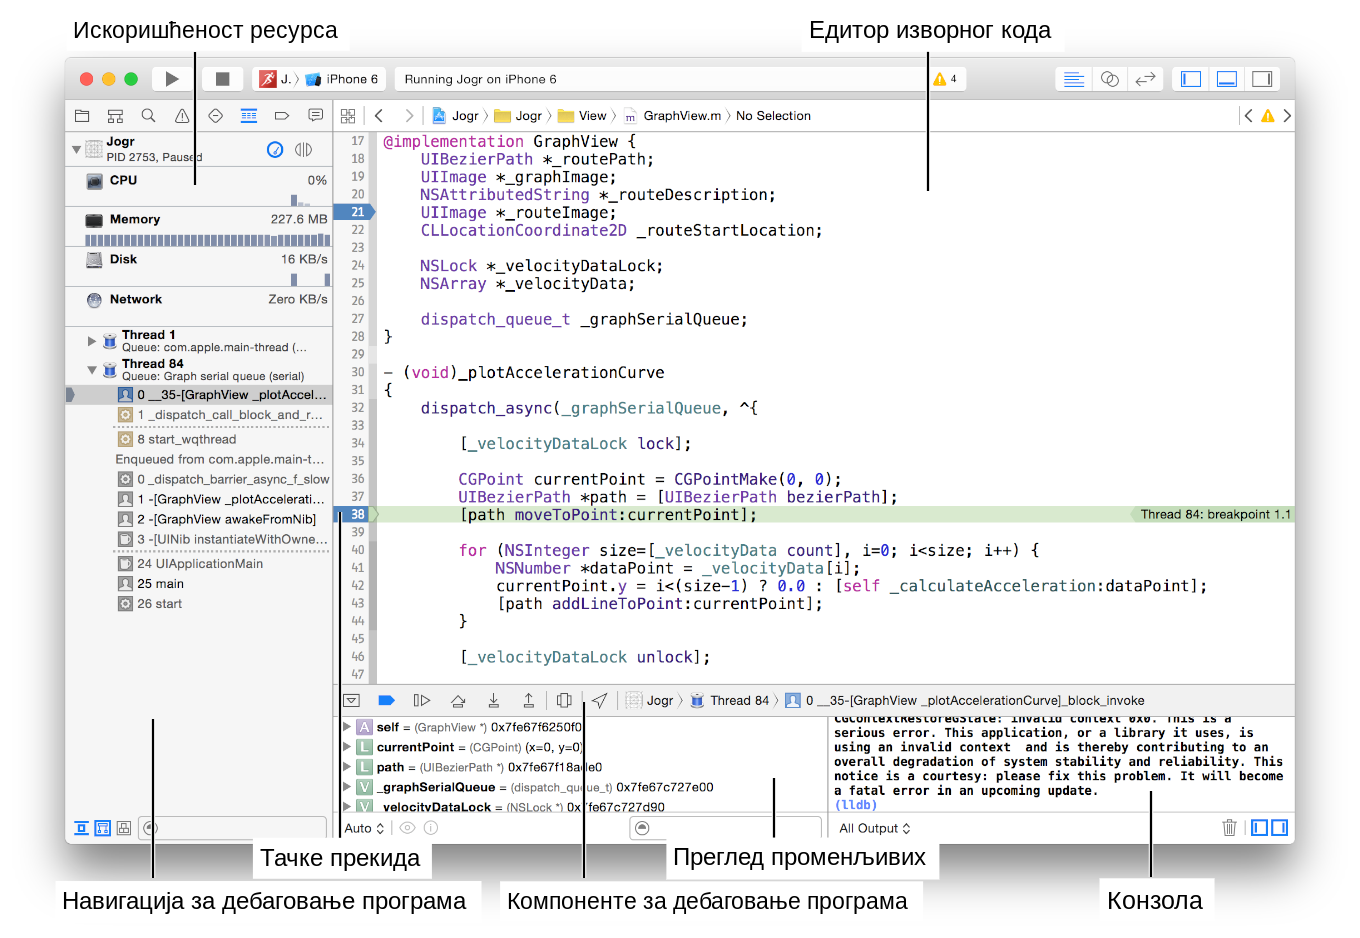
\includegraphics[width=\textwidth]{slike/xcode.png}
    \end{center}
    \caption{Изглед интегрисаног графичког корисничког окружења {\em Xcode}}
    \label{fig:xcode}
\end{figure}

\subsection{Microsoft Visual Studio Debugger - MVSD}

{\em MVSD} је дебагер доступан за коришћење из развојног 
окружења {\em Visual Studio}. Како је у питању комерцијални
софтверски производ, није познато превише детаља око интерне
имплементације и архитектуре у односу на развојно окружење.
{\em MVSD} је апстрахован кроз {\em Visual Studio} и ретко
се посматра као одвојени систем или алат из угла корисника. 
Односно, на њега се више посматра као функционалност
коју пружа развојно окружење и није доступан за коришћење 
из других алата \cite{msvd}. На слици \ref{fig:msvd} је приказан
пример употребе овог дебагера.

Подржане су практично све најчешће функционалности дебагера
као што су условне тачке прекида, праћење тока извршавања програма, 
приказ садржаја променљивих, извршавање корак по корак, 
евалуација израза, позивање функција приликом дебаговања, 
постављање тачака посматрања, повезивање на процес у извршавању
и слично \cite{msvd}. 

\begin{figure}
    \begin{center}
        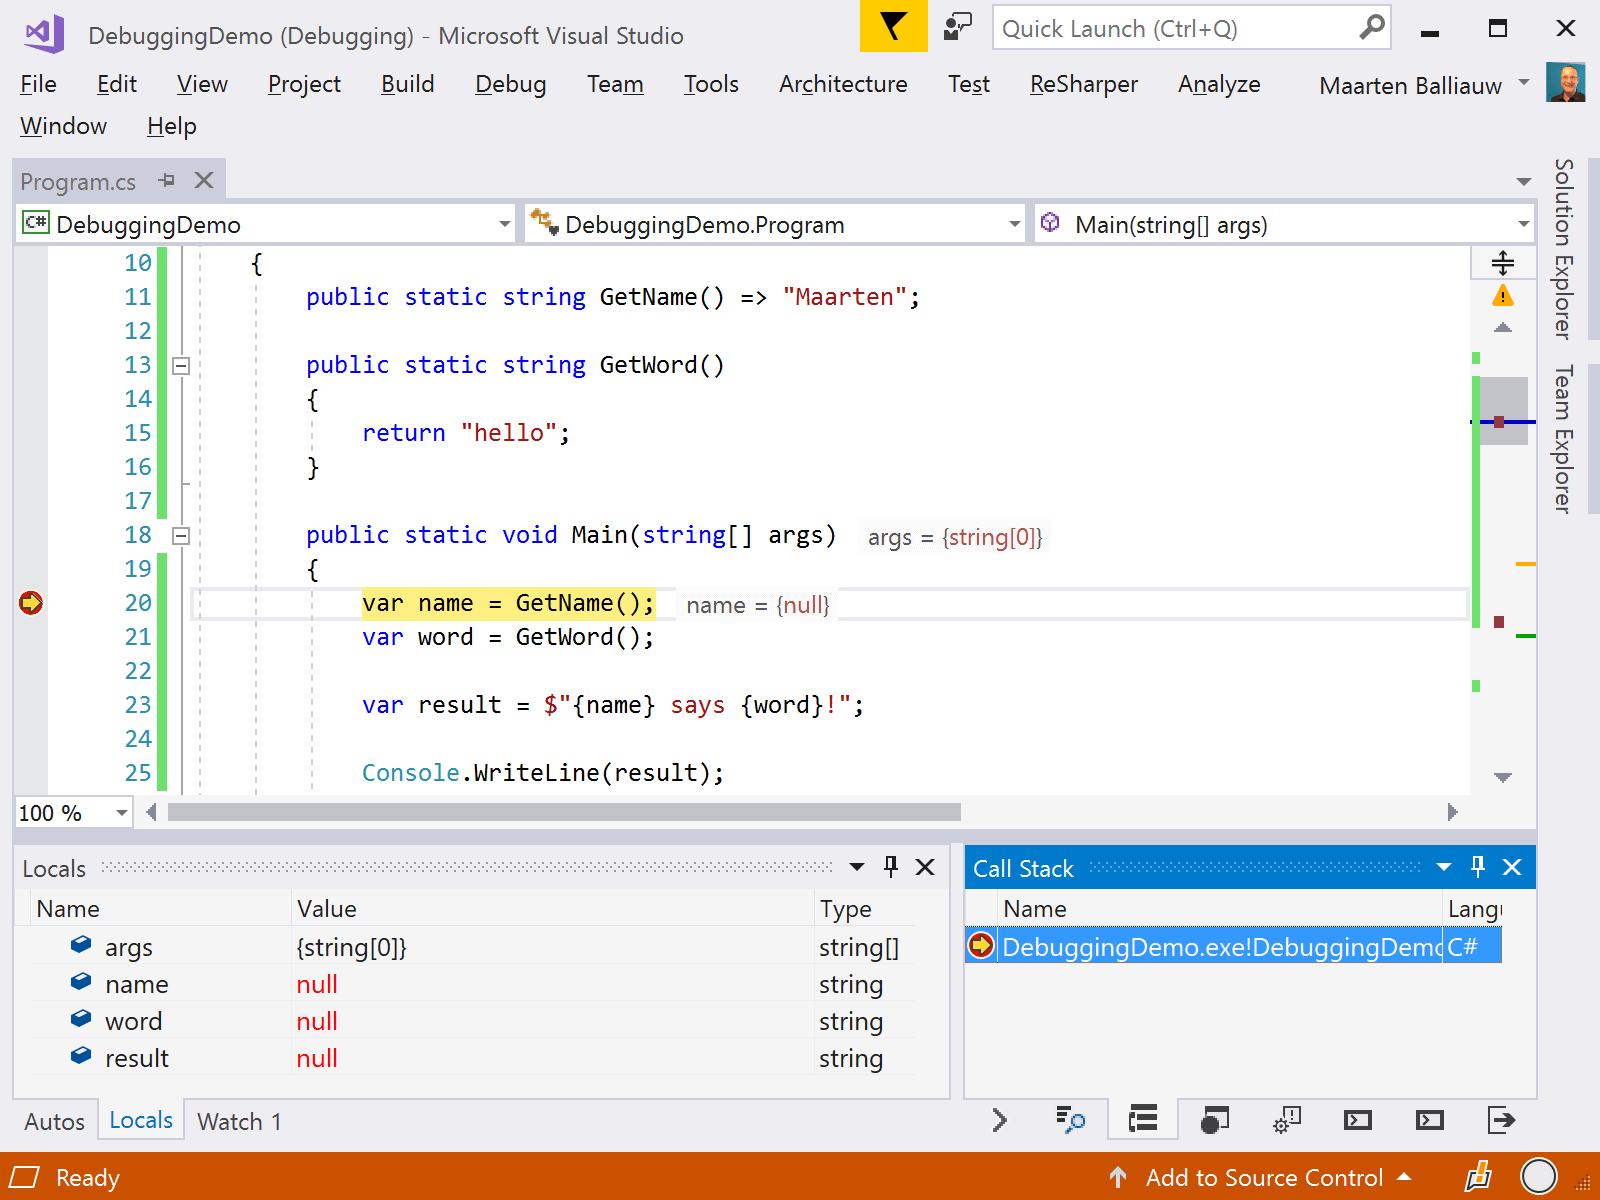
\includegraphics[width=\textwidth]{slike/msvd.png}
    \end{center}
    \caption{Пример коришћења {\em Visual Studio} дебагера}
    \label{fig:msvd}
\end{figure}

\subsection{WinDBG}

{\em WinDBG} је дебагер који развија компанија {\em Microsoft} 
за платформу {\em Windows}. Његове најчешће намене јесу дебаговање 
процеса на страни кернела као и драјвера. Постоји и програм са истим 
именом који пружа графички кориснички интерфејс за коришћење овог 
дебагера. У пракси је ово дебагер који се користи за дебаговање 
проблема који се популарно зову плави екран смрти (eng. Blue Screen of Death - BSOD)
и представљају ситуације у којимa оперативни систем {\em Windows}
престане са радом услед озбиљне грешке.
Пример оваквог проблема дат је на слици \ref{fig:blueScreen}.
Постоји и подршка за проширивање функционалности овог дебагера 
путем прикључака који се повезују са алатом као библиотеке са 
динамичким повезивањем (eng. Dynamic Linkable Library - DLL) \cite{windbg}.

\begin{figure}
    \begin{center}
        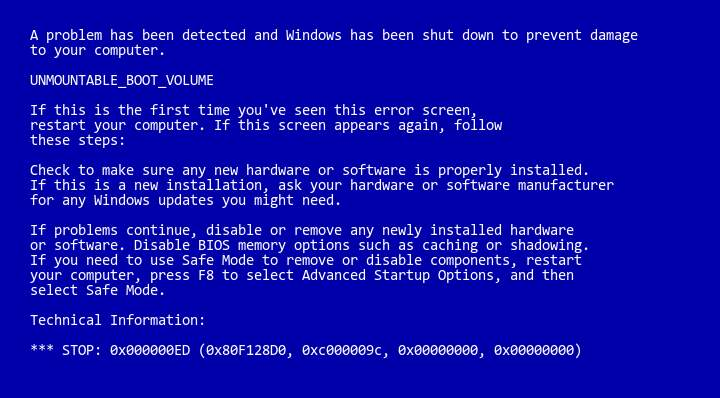
\includegraphics[width=\textwidth]{slike/plavi_ekran_smrti.jpg}
    \end{center}
    \caption{{\em Blue Screen of Death} - екрански приказ након фаталне 
    системске грешке на {\em Microsoft Windows} оперативним системима}
    \label{fig:blueScreen}
\end{figure}

Једна од разлика у односу на {\em MSVD} јесте у томе што је 
овај алат само дебагер који није директно интегрисан
у развојно окружење, иако наравно, постоји подршка за 
његово коришћење и у оквиру {\em Visual Studio} алата.
Услед тога, алат заузима драстично мање меморије на диску
и брже и лакше се покреће у односу на целокупан
систем који представља {\em Visual Studio}. Постоје и 
функционалности које {\em WinDBG} поседује које нису доступне
кроз {\em MSVD} дебагер. Више о овим разликама и 
функционалностима је доступно у табели \ref{tab:summary}.

Компанија {\em Microsoft} je 2017. године објавила нову 
верзију овог дебагера под називом {\em WinDBG Preview}
која је донела побољшања за графички кориснички интерфејс и 
пре свега подршку за дебаговање са такозваним
{\em путовањем кроз време} (eng. Time Travel Debugging - TDD).
Основна идеја овакве врсте дебаговања је у томе
да се приликом извршавања процеса сачувају све неопходне 
информације како би се после тај процес могао дебаговати
унапред и уназад \cite{tdd}. Ово може бити посебно корисно за 
дебаговање програма пре него што је дошло до његовог пуцања
када у класичном дебаговању процес више није доступан за 
дебаговање \cite{windbgx}. На слици \ref{fig:windbg-preview} 
је приказан алат {\em WinDBG Preview}, а на слици \ref{fig:windbg-tdd} 
је приказана слика на којој се види како се може покренути 
програм са укљученом подршком за ТДД дебаговање
кроз алат {\em WinDBG Preview}.

\begin{figure}
    \begin{center}
        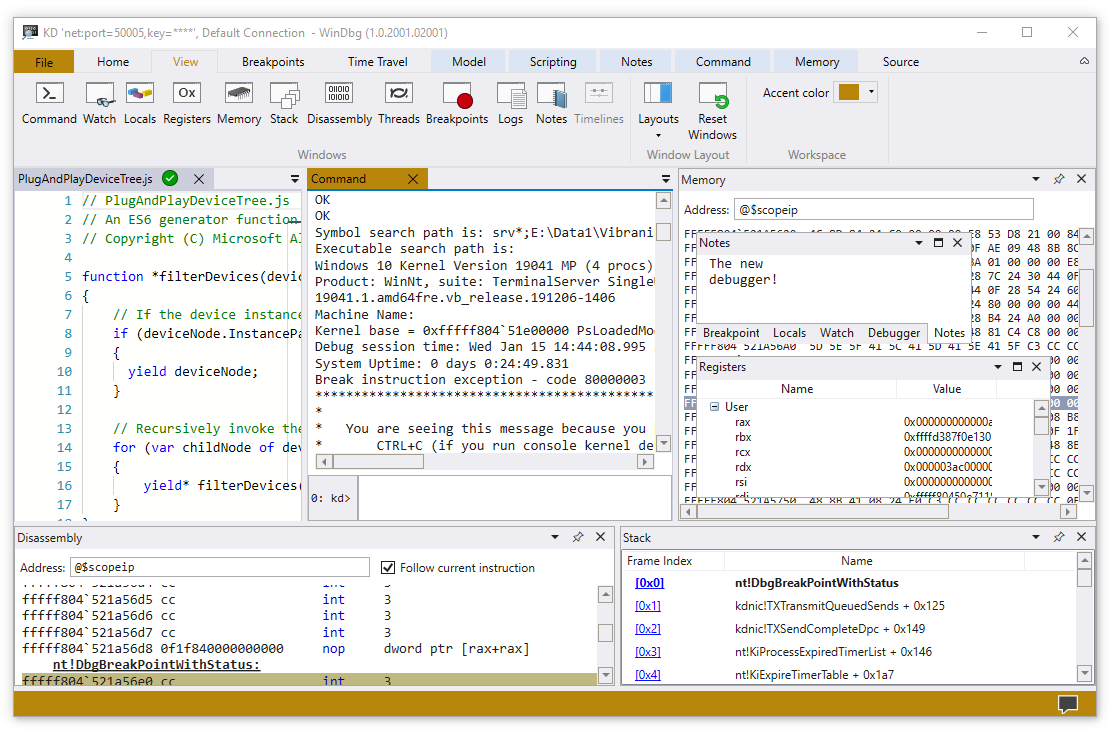
\includegraphics[width=\textwidth]{slike/windbgx.png}
    \end{center}
    \caption{Пример коришћења {\em WinDBG} дебагера}
    \label{fig:windbg-preview}
\end{figure}

\begin{figure}
    \begin{center}
        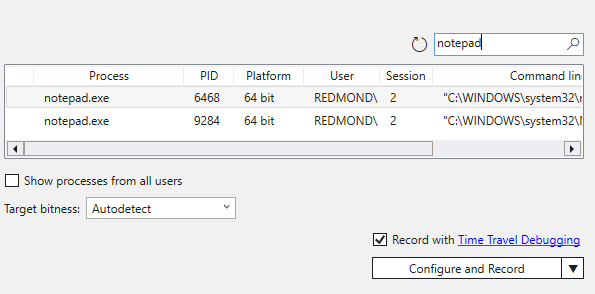
\includegraphics[width=\textwidth]{slike/windbgx_tdd.png}
    \end{center}
    \caption{Пример коришћења {\em TDD} дебаговања у алату {\em WinDBG Preview}}
    \label{fig:windbg-tdd}
\end{figure}

\subsection{Java debugger - JDB}

Јава debager (eng. ~{\em Java debugger}), најчешће скраћено само {\em JDB}, је алат командне линије 
за дебаговање програма имплеменитраних у језику Јава.
Еквивалент је {\em GDB} дебагеру за Јава виртуелну машину и долази испоручен у оквиру
развојног пакета језика Јава (eng. ~{\em Java SE Development Kit}).
Овај алат имплементира такозвану архитектуру програма за дебаговање
{\em Java} платформе (eng. ~{\em Java Platform Debugger Architecture}) која је приказана на слици \ref{fig:jdb}.
Ова архитектура састоји се из три главне компоненте \cite{oracle}:
\begin{itemize}
 \item Интерфејс Јава виртуелне машине, која омогућава преглед и
 дебаговање стања апликације која се извршава на виртуелној машини.
 \item Интерфејс за дебаговање, који пружа информације корисне дебагерима
 и сличним системима којима је потребан приступ стању виртуелне машине у 
 току извршавања (често удаљено).
 \item Протокол који се користи за комуникацију између дебагера и Јава
 виртуелне машине коју дебагује. Постојање овог протокола може омогућити
 дебагеру да ради на различитим процесима истог система или на неком удаљеном
 рачунару.
\end{itemize}

\begin{figure}
    \begin{center}
        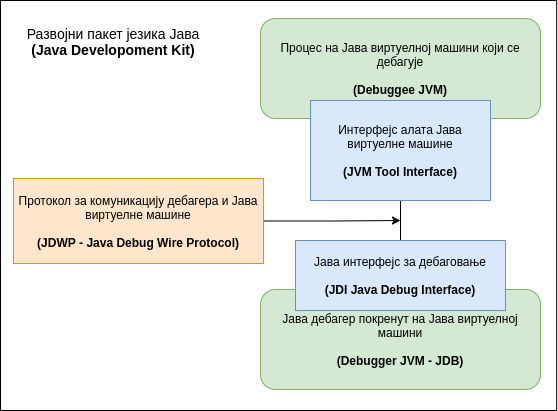
\includegraphics[width=\textwidth]{slike/javajdb.png}
    \end{center}
    \caption{Архитектура програма за дебаговања {\em Java} платформе}
    \label{fig:jdb}
\end{figure}

Када се Јава дебагер покрене и проследи му се име класе, 
он покреће другу копију Јава интерпретера. {\em JDB} је, дакле,
сам по себи такође Јава програм који се извршава коришћењем
додељене копије интерпретера. Овај нови интерпретер учитава фајл који
садржи наведену класу и зауставља се ради дебаговања пре извршавања првог
бајт кода \cite[Chapter 16]{javaInANutshell}. Овај дебагер се такође може
покренути тако да се накачи на процес који се већ извршава.

Након што је дебаговање започето, може се извршити велики број команди 
\cite[Chapter 16]{javaInANutshell}.
Међу њима је {\em catch} команда помоћу које се може изазвати прекид извршавања сваки
пут када се подигне изузетак. Још неке занимљиве опције које нуди овај
дебагер су могућност позивања сакупљача отпадака, приказ искоришћености меморије
као и промена тренутне нити извршавања.

\subsection{Bash debugger - bashdb}

Основна употреба дебагера за скрипт језик јесте да омогући
да се види шта се догађа унутар саме скрипте у току њеног извршавања.
Иако је ово дебагер командне линије, за њега постојe прикључци 
који омогућавају коришћење кроз {\em Visual Studio Code} и 
кроз алате компаније {\em JetBrains}. Такође и алат {\em DDD} поменут у секцији
\ref{sec:gdb}, нуди подршку за коришћење овог дебагера кроз графички кориснички
интерфејс \cite{bashDB}. На слици \ref{fig:bashdbVscode} приказан је пример коришћења алата {\em bashdb}
у оквиру едитора {\em Visual Studio Code}.

\begin{figure}
    \begin{center}
        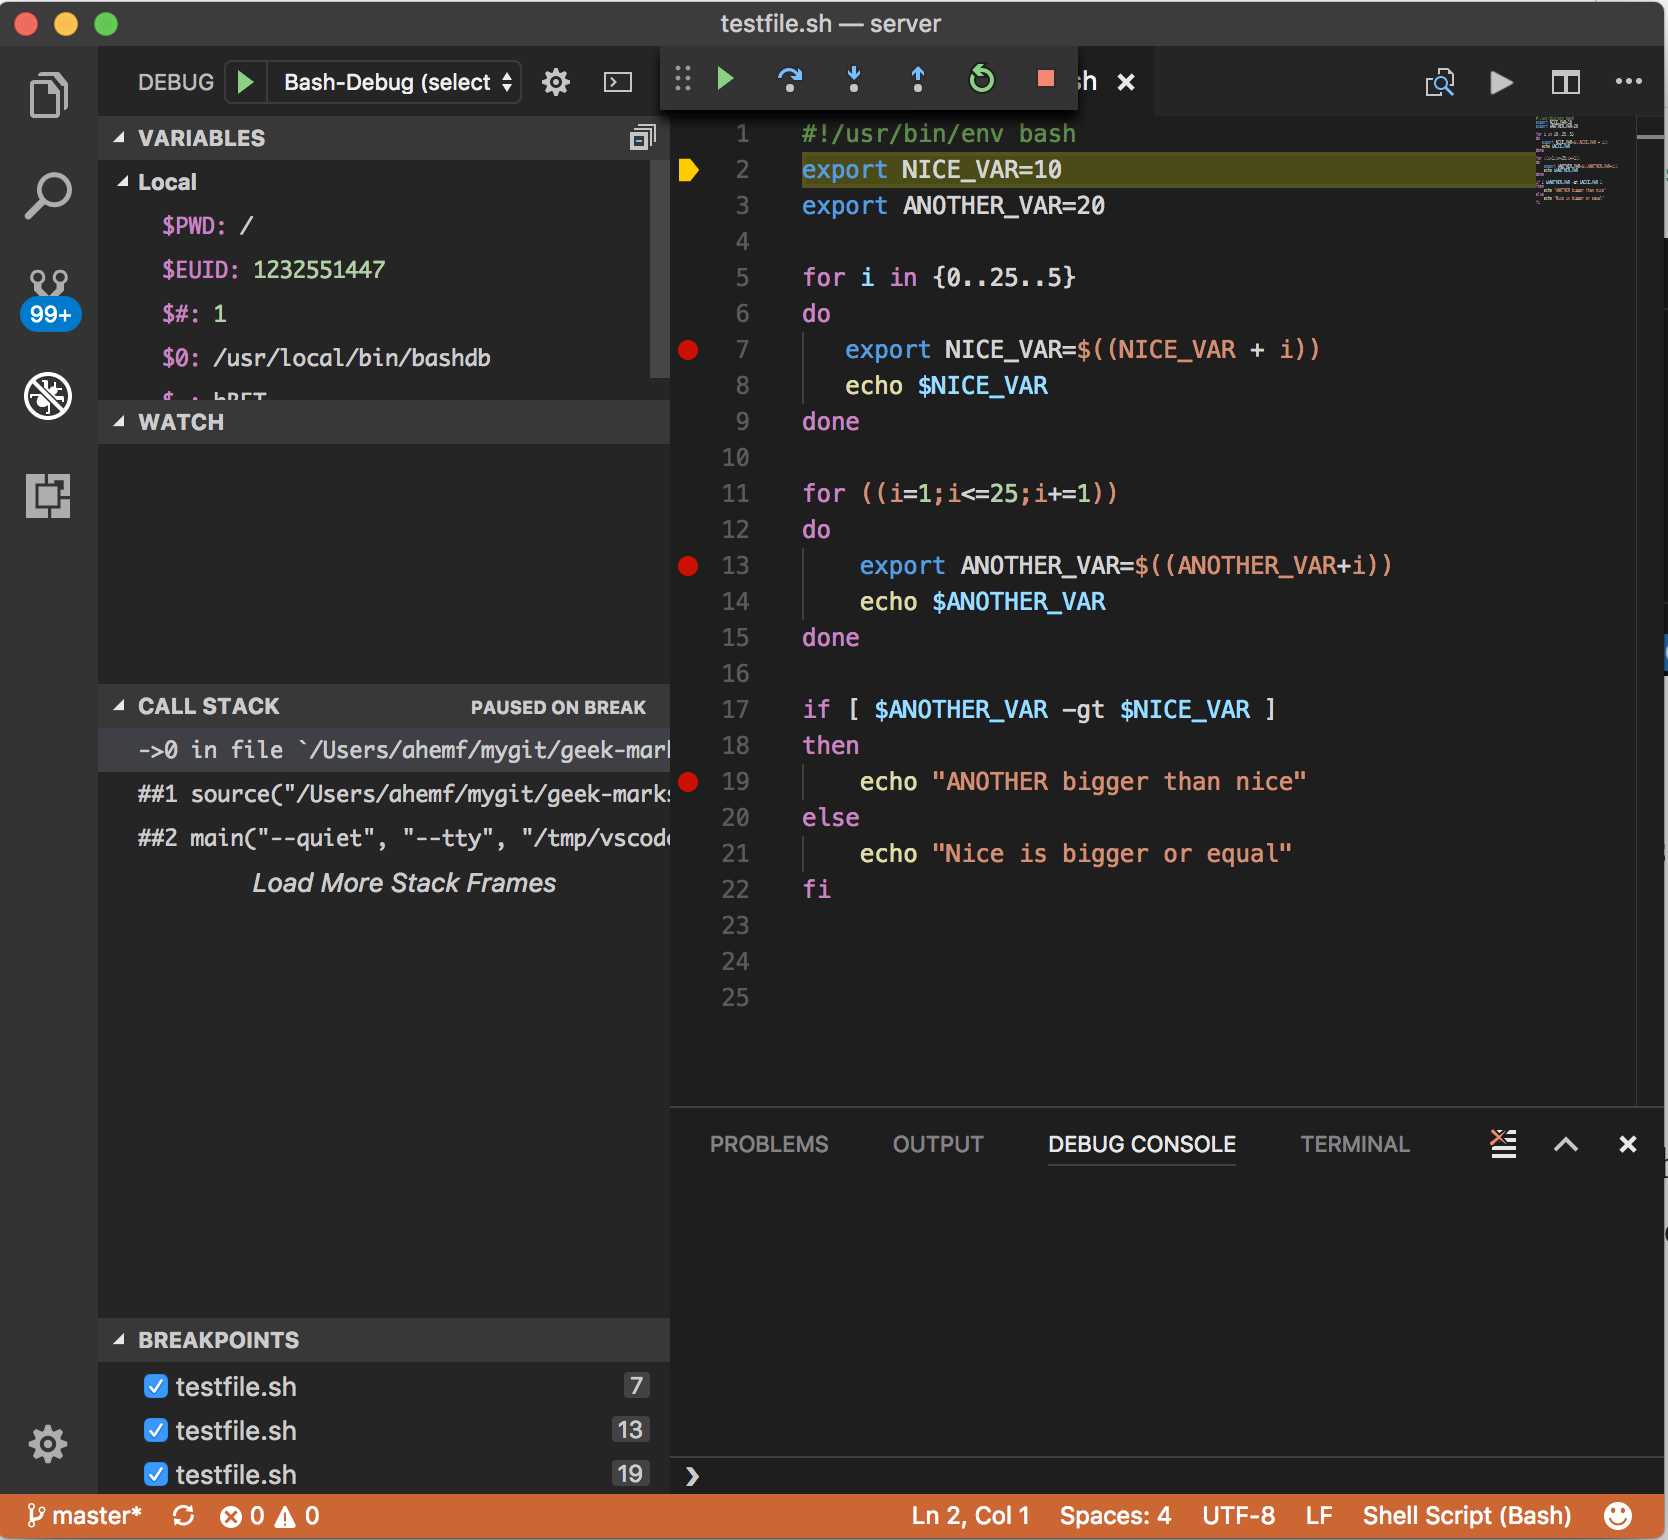
\includegraphics[scale=0.17]{slike/bashdb_vscode.png}
    \end{center}
    \caption{Пример коришћења {\em bashdb} дебаговања у алату {\em Visual Studio Code}}
    \label{fig:bashdbVscode}
\end{figure}

{\em BashDB} има четири главна циља у помоћи за дебаговање
{\em Bash} скрипти. Ти циљеви су:

\begin{itemize}
 \item Покретање жељене скрипте и дефинисање свега што би могло утицати на понашање
 \item Заустављање извршавања скрипте уколико је испуњен дефинисани услов
 \item Испитивање шта се догодило након што је заустављено извршавање скрипте
 \item Измена саме скрипте, како би се исправили ефекти указаног бага
\end{itemize}

Функционалности које су подржане како би омогућиле извршавање
ових циљева су могућност постављања тачака прекида, инспекција
вредности променљивих, кретање уназад али и кретање кроз скрипту
корак по корак \cite{bashDB}. Другим речима, пружа неке основне могућности које су
за очекивати дебагерима за на пример програмске језике {\em C} или {\em C++}.
Такође, подржана је и могућност постављања тачки посматрања да би се
видело да ли и када се нека променљива мења. Постоји и команда
\texttt{watche} која омогућава прекид извршавања кад год прослеђени израз
буде евалуиран као тачан.

\subsection{The Firefox JavaScript Debugger}

{\em Firefox} алати за развој (eng. ~{\em Firefox Developer Tools})
представљају скуп алата који су уграђени у веб прегледач под
називом {\em Firefox}. Састоје се од неколико различитих алата који
омогућавају испитивање, мењање и дебаговање {\em HTML, CSS} и 
{\em JavaScript} кода. Међу њима је, поред веб конзоле, алата за
мењање поравнања и садржаја, алата за праћење перформанси и других,
и дебагер за програмски језик {\em JavaScript} \cite{jsDevTools}.

Овај дебагер се може користити за дебаговање кода који се извршава 
локално, на истој машини, али и за дебаговање кода који се налази 
на некој удаљеној машини. То значи да је могуће користити {\em 
Firefox JavaScript} дебагер на локалном рачунару да се дебагује неки веб сајт
или веб апликација која се извршава у другим прегледачима или 
окружењима за извршавање (eng. ~{runtime}), на пример на мобилном
телефону који је повезан преко УСБ кабла. Пример коришћења дат је на
слици \ref{fig:jsDebugger}.

\begin{figure}
    \begin{center}
        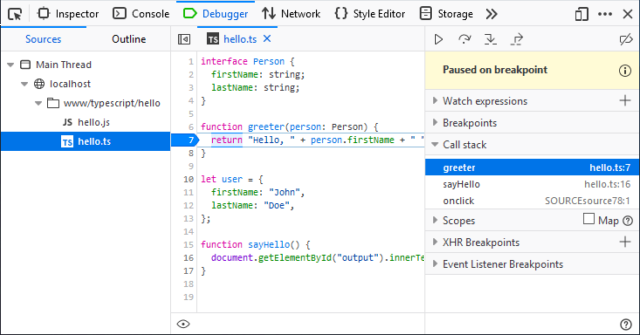
\includegraphics[width=\textwidth]{slike/javascript_debager.png}
    \end{center}
    \caption{Пример употребе {\em JavaScript} дебагера у {\em Firefox} веб прегледачу}
    \label{fig:jsDebugger}
\end{figure}

Као и већина претходно изнетих дебагера и {\em 
Firefox JavaScript} дебагер нуди мноштво функционалности за олакшавање
проналажења узрока грешака. Неке од њих су омогућавање постављања 
тачака прекида на промене {\em DOM} стабла, затим паузирање извршавања
када се деси неки очекивани догађај и паузирање када се подигне неки
изузетак. Више о додатним могућностима може се видети на \cite{firefoxDebugger}.

\section{Сумарни преглед могућности}

Сваки од дебагера изложених у поглављу \ref{sec:debuggerOverview} има
своје предности, које потичу од специфичности система или програмског језика
за који су првенствено намењени. Међутим, већина њих ипак дели одређени подскуп
функционалности.

Како би се стекао осећај о старости, одржавању и томе за шта је намењен који дебагер,
у табели \ref{tab:about} приказане су неке основне информације о сваком од изложених дебагера.
У табели \ref{tab:summary} дат је упоредни приказ особина које би могле бити корисне,
а опет их дели већи подскуп изложених дебагера. Технике дебаговања које
су описане у поглављу \ref{sec:whatCanDebuggersDo} издвојене су у посебну табелу
\ref{tab:techniques} и приказане за сваки од дебагера шта од њих подржава.


\begin{table}[ht!]
    \begin{center}
        \caption{Техничке особине изложених дебагера}
        \begin{tabular}{|c|c|c|c|c|c|} \hline
        \diagbox{Дебагер}{Особина} & \thead{Прва \\ верзија} & \thead{Платформе} & \thead{Програмски \\ језици} & \thead{Последња \\ верзија} \\ \hline
        
        \textbf{GDB} & 1986. & \thead{{\em UNIX} \\ системи, \\ {\em Windows}} & \thead{\em C, C++, \\ {\em D, Fortran}, \\ {\em Pascal}, \\ {\em Modula-2}, \\ {\em Ada}} & \thead{Окт 2020.} \\ \hline
        
        \textbf{LLDB} & 2012. & \thead{{\em Linux} \\ {\em Windows} \\ {\em macOS, iOS} \\ {\em watchOS}, \\ {\em FreeBSD}} & \thead{\em C, C++, \\ {\em Objective-C}, \\ {\em Objective-C++}} & Окт 2020. \\ \hline
        
        \textbf{MVSD} & 1995. & {\em Windows} & \thead{\em C\#, C++, \\ {\em Visual Basic, F\#}, \\ Python, JavaScript} & Јан 2020. \\ \hline
        
        \textbf{WinDBG} & ? & {\em Windows} & {\em C, C++} & Aпр 2020. \\ \hline
        
        \textbf{JDB} & 2000. & \thead{\em Windows, \\ {\em macOS}, \\ {\em Linux}, \\ {\em Solaris}} & \thead{Java} & Сеп 2020. \\ \hline
        
        \textbf{BashDB} & 2003 & {\em UNIX} системи & {\em Bash} & Дец 2019. \\ \hline
        
        \thead{\textbf{Firefox} \\ \textbf{JavaScript} \\ \textbf{дебагер}} & 2011 & \thead{{\em Windows} \\ {\em Linux} \\ {\em macOS}} & \thead{{\em JavaScript}, \\ {\em TypeScript}} & Сеп 2020. \\ \hline
        \end{tabular}
        \label{tab:about}
    \end{center}
\end{table}


\begin{table}[ht!]
    \begin{center}
        \caption{Упоредни реглед могућности изложених дебагера}
        \begin{tabular}{|c|c|c|c|c|c|c|} \hline
        \diagbox{Дебагер}{Особина} & \thead{Условне \\ тачке \\ прекида} & \thead{Тачке \\ посма- \\ трања} & \thead{Евалу- \\ ација \\ израза} & \thead{Праћење \\ изузетака} & \thead{Више- \\ нитне \\ апликације}\\ \hline
        
        \textbf{GDB} & \cmark & \cmark & \cmark & \cmark & \cmark \\ \hline
        
        \textbf{LLDB} & \cmark  & \cmark & \cmark & \cmark & \cmark \\ \hline
        
        \textbf{MVSD} & \cmark  & \cmark & \cmark & \cmark & \cmark \\ \hline
        
        \textbf{WinDBG} & \cmark  & \cmark & \cmark & \cmark & \cmark \\ \hline
        
        \textbf{JDB} & \xmark  & \cmark & \cmark & \cmark & \cmark \\ \hline
        
        \textbf{BashDB} & \cmark & \cmark & \cmark & \xmark & \xmark \\ \hline
        
        \thead{\textbf{Firefox} \\ \textbf{JavaScript} \\ \textbf{дебагер}} & \cmark & \cmark & \cmark & \cmark & \cmark\\ \hline
        \end{tabular}
        \label{tab:summary}
    \end{center}
\end{table}

\begin{table}[ht!]
    \begin{center}
        \caption{Упоредни реглед техника које подржавају изложени дебагери}
        \begin{tabular}{|c|c|c|c|c|c|c|} \hline
        \diagbox{Дебагер}{Техника} & \thead{Дебаговање \\ уназад} & \thead{Удаљено \\ дебаговање} & \thead{\em Post- \\ {\em mortem} \\ дебаговање}\\ \hline
        
        \textbf{GDB} & \cmark  & \cmark  & \cmark  \\ \hline
        
        \textbf{LLDB} & \cmark  & \cmark & \cmark  \\ \hline
        
        \textbf{MVSD} & \cmark  & \cmark & \cmark  \\ \hline
        
        \textbf{WinDBG} & \cmark  & \cmark & \cmark  \\ \hline
        
        \textbf{JDB} & \xmark  & \cmark & \xmark \\ \hline
        
         \textbf{BashDB} & \xmark & \cmark & \xmark \\ \hline
        
        \thead{\textbf{Firefox} \\ \textbf{JavaScript} \\ \textbf{дебагер}} & \xmark & \cmark & \cmark \\ \hline
        \end{tabular}
        \label{tab:techniques}
    \end{center}
\end{table}


\section{Закључак}
\label{sec:conclusion}

Комплекност и количина написаног софтвера расте из године у
годину услед све већег броја рачунара
који су у оптицају и који се уграђују у уређаје као што су 
аутомобили, авиони, телевизори, роботи
и слично. Откривање, анализа и отклањање багова додатно
добијају на значају у жељи да се софтверски
развојни процес учини максимално ефикасним и 
квалитетним као и да се минимизују трошкови и ризици.
Дебагери су међу најважнијим алатима за остваривање 
ових циљева и интензивно се користе.

Ови интересантни алати често поседују ефекат који
није реткост и за оперативне системе - бивају узети здраво за готово.
Очекује се да су ту, да раде брзо и ефикасно, а ретко се 
обрати пажња на њихову комплекност,
корисност и начин на који раде. Интересантно је приметити 
да је дебагер производ рада једног или више
програмера, да му је улаз програм, а да је корисник 
дебагера првенствено и једино програмер.
Односно, дебагер као резултат развојног процеса 
би требао да буде изузетно квалитетан јер сви они
који учествују у његовом развијању поседују озбиљно 
разумевање својих корисника као и њихових
потреба и проблема.

Из описаног издвојеног подскупа дебагера, 
изводи се закључак да иако сваки од њих има своје 
специфичности, ипак на крају већина ових алата пружа
сличан скуп функционалности. То, уз чињеницу да су
се аутори сваког од њих трудили да задрже сличан начин
употребе, омогућава програмерима
да, уз познавање једног од ових алата, могу једноставно и брзо
да пређу на коришћење другог алата у тренутку када им
је то неопходно. Ово важи како за алате командне линије, 
тако и за оне који имају и графичко корисничко окружење.

\newpage

\addcontentsline{toc}{section}{Литература}
\appendix
\bibliography{literatura} 
\bibliographystyle{plain}

\end{document}
